%%%%%%%%%%%%%%%%%%%%%%%%%%%%%%%%%%%%%%%%%%%%%%%%%%%
% GammaLib Software Design Description
%%%%%%%%%%%%%%%%%%%%%%%%%%%%%%%%%%%%%%%%%%%%%%%%%%%

%%%%%%%%%%%%%%%%%%%%%%%%%%%%%%%%%%%%%%%%%%%%%%%%%%%
% Definitions for manual package
%%%%%%%%%%%%%%%%%%%%%%%%%%%%%%%%%%%%%%%%%%%%%%%%%%%
\newcommand{\task}{\mbox{GammaLib}}
\newcommand{\this}{\mbox{\tt \task}}
\newcommand{\shorttype}{\mbox{SDD}}
\newcommand{\doctype}{\mbox{Software Design Description}}
\newcommand{\version}{\mbox{draft}}
\newcommand{\calendar}{\mbox{23 May 2010}}
\newcommand{\auth}{\mbox{J\"urgen Kn\"odlseder}}
\newcommand{\approv}{\mbox{J\"urgen Kn\"odlseder}}


%%%%%%%%%%%%%%%%%%%%%%%%%%%%%%%%%%%%%%%%%%%%%%%%%%%
% Document definition
%%%%%%%%%%%%%%%%%%%%%%%%%%%%%%%%%%%%%%%%%%%%%%%%%%%
\documentclass{article}[12pt,a4]
\usepackage{epsfig}
\usepackage{manual}


%%%%%%%%%%%%%%%%%%%%%%%%%%%%%%%%%%%%%%%%%%%%%%%%%%%
% Begin of document body
%%%%%%%%%%%%%%%%%%%%%%%%%%%%%%%%%%%%%%%%%%%%%%%%%%%
\begin{document}
\frontpage


%%%%%%%%%%%%%%%%%%%%%%%%%%%%%%%%%%%%%%%%%%%%%%%%%%%
% Introduction
%%%%%%%%%%%%%%%%%%%%%%%%%%%%%%%%%%%%%%%%%%%%%%%%%%%
\section{Introduction}

%%%%%%%%%%%%%%%%%%%%%%%%%%%%%%%%%%%%%%%%%%%%%%%%%%%
\subsection{Design Overview}

%%%%%%%%%%%%%%%%%%%%%%%%%%%%%%%%%%%%%%%%%%%%%%%%%%%
\subsection{Requirements Traceability Matrix}


%%%%%%%%%%%%%%%%%%%%%%%%%%%%%%%%%%%%%%%%%%%%%%%%%%%
% System architectural design
%%%%%%%%%%%%%%%%%%%%%%%%%%%%%%%%%%%%%%%%%%%%%%%%%%%
\section{System Architectural Design}

%%%%%%%%%%%%%%%%%%%%%%%%%%%%%%%%%%%%%%%%%%%%%%%%%%%
\subsection{Chosen System Architecture}

The \this\ is designed for Linux, Unix and MacOS~X systems and compiles under
32 Bit and 64 Bit.

%%%%%%%%%%%%%%%%%%%%%%%%%%%%%%%%%%%%%%%%%%%%%%%%%%%
\subsection{Discussion of Alternative Designs}

%%%%%%%%%%%%%%%%%%%%%%%%%%%%%%%%%%%%%%%%%%%%%%%%%%%
\subsection{System Interface Description}

The \this\ is designed as C++ API library of which all modules are designed as classes.
A Python interface allows scripting of library components.


%%%%%%%%%%%%%%%%%%%%%%%%%%%%%%%%%%%%%%%%%%%%%%%%%%%
% Detailed Description of Components
%%%%%%%%%%%%%%%%%%%%%%%%%%%%%%%%%%%%%%%%%%%%%%%%%%%
\section{Detailed Description of Components}

%%%%%%%%%%%%%%%%%%%%%%%%%%%%%%%%%%%%%%%%%%%%%%%%%%%
\subsection{Applications}

%%%%%%%%%%%%%%%%%%%%%%%%%%%%%%%%%%%%%%%%%%%%%%%%%%%
\subsubsection{{\tt GApplication}}

%%%%%%%%%%%%%%%%%%%%%%%%%%%%%%%%%%%%%%%%%%%%%%%%%%%
\subsubsection{{\tt GPars}}

%%%%%%%%%%%%%%%%%%%%%%%%%%%%%%%%%%%%%%%%%%%%%%%%%%%
\subsubsection{{\tt GLog}}


%%%%%%%%%%%%%%%%%%%%%%%%%%%%%%%%%%%%%%%%%%%%%%%%%%%
\subsection{Skymaps}

%%%%%%%%%%%%%%%%%%%%%%%%%%%%%%%%%%%%%%%%%%%%%%%%%%%
\subsubsection{{\tt GSkymap}}

The {\tt GSkymap} class holds a single skymap (or a set of skymaps with identical coordinates)
in a specific world coordinate projection (see {\tt GWcs}).
Three different constructors exist:
\begin{verbatim}
  GSkymap(void);
  GSkymap(std::string wcs, std::string coordsys, int nside, std::string ordering,
          int nmaps = 1);
  GSkymap(std::string wcs, std::string coordsys, GSkyDir dir, int nlon, int nlat, 
          double dlon, double dlat, int nmaps = 1);
\end{verbatim}
The first one creates an instance of an empty skymap.

The second is for creating an instance of a Healpix skymap.
Here
{\tt wcs} needs to be {\tt HPX} (we add this for consistency),
{\tt coordsys} is the coordinate system (see below),
{\tt nside} is the $N_{side}$ parameter,
{\tt ordering} is the pixel ordering (either {\tt RING} or {\tt NESTED}, case independent),
and
{\tt nmaps} gives the number of maps in a set (defaults to 1 if not given).

The third is for creating an instance of any other type of skymap.
Here
{\tt wcs} is the projection of the skymap (see {\tt GWcs}),
{\tt coordsys} is the coordinate system (see below),
{\tt dir} is the position of the map centre,
{\tt nlon} is the number of pixels in longitude,
{\tt nlat} is the number of pixels in latitude,
{\tt dlon} is the pixel size in longitude (in units of degrees),
{\tt dlat} is the pixel size in latitude (in units of degrees),
and
{\tt nmaps} gives the number of maps in a set (defaults to 1 if not given).

Two coordinate systems are implemented ({\tt coordsys}):
{\tt GAL} indicates the galactic system (galactic longitude and latitude), and
{\tt CEL} indicates equatorial or celestial system (Right Ascension and declination).

The following methods are defined for {\tt GSkymap}:
\begin{verbatim}
  void        read(std::string filename);     //!< Read skymap from FITS file
  void        read(const GFitsHDU* hdu);      //!< Read skymap from FITS HDU
  void        write(std::string filename);    //!< Write skymap into FITS file
  void        write(GFitsHDU* hdu);           //!< Write skymap into FITS HDU
  std::string ordering(void) const;           //!< Returns Healpix ordering ("" if not Healpix)
  std::string coordsys(void) const;           //!< Returns coordinate system
  GSkyDir     pix2dir(const int& pix);        //!< Convert pixel index to sky direction
  int         dir2pix(GSkyDir dir) const;     //!< Convert sky direction to pixel index
  double      omega(const int& pix);          //!< Return solid angle of pixel (in steradian)
  int         npix(void) const;               //!< Return number of pixels in image
  int         nside(void) const;              //!< Return number of sides (0 if not Healpix)
  int         nlon(void) const;               //!< Return number of longitude pixels (0 if Healpix)
  int         nlat(void) const;               //!< Return number of latitude pixels (0 if Healpix)
  void        ordering(std::string ordering); //!< Change Healpix ordering (RING or NESTED)
  void        coordsys(std::string coordsys); //!< Change coordinate system (CEL or GAL)
  void        nside(int nside);               //!< Change Healpix N_side parameter
  void        rebin(int nlon, int nlat);      //!< Change number of longitude/latitude pixels
  void        smooth_gaussian(double sigma);  //!< Smooth skymap using Gaussian kernel
\end{verbatim}

The {\tt GSkymap} class contains:
\begin{verbatim}
  GWcs*   m_wcs;     //!< Pointer to World Coordinate System projection
  double* m_pixels;  //!< Pointer to sky map pixels
\end{verbatim}

Note that the skymap is internally stored in a double precision array.
The class may eventually by extended to also handle other storage types.
Alternatively, the class could also be implemented as a template class.


%%%%%%%%%%%%%%%%%%%%%%%%%%%%%%%%%%%%%%%%%%%%%%%%%%%
\subsubsection{{\tt GWcs}}

Virtual base class that implements projections from sky coordinates into a vector of
image pixels.
The class follows the World Coordinate System (WCS) convention.

The following pure virtual methods are defined for {\tt GWcs}:
\begin{verbatim}
  void    read(const GFitsHDU* hdu);     //!< Read projection information from FITS header
  void    write(GFitsHDU* hdu);          //!< Write projection information to FITS header
  GSkyDir pix2dir(const int& pix);       //!< Convert pixel index to sky direction
  int     dir2pix(GSkyDir dir) const;    //!< Convert sky direction to pixel index
  double  omega(const int& pix);         //!< Return solid angle of pixel (in steradian)
  int     npix(void) const;              //!< Return number of pixels in image
  int     naxes(void) const;             //!< Return number of image axes
  int     naxis(const int& axis) const;  //!< Return number of pixels in specified axis
\end{verbatim}

The HEALPix projection (as a general class of spherical projections) is represented by the 
keyword HPX in the FITS standard for writing astronomical data files.


%%%%%%%%%%%%%%%%%%%%%%%%%%%%%%%%%%%%%%%%%%%%%%%%%%%
\subsection{Observation handling}

%%%%%%%%%%%%%%%%%%%%%%%%%%%%%%%%%%%%%%%%%%%%%%%%%%%
\subsubsection{{\tt GObservation}}

Observation handling provides an abstract interface to gamma-ray observations of all kinds
without any reference to instrument specific properties.
An observation is defined as a given period in time during which data are acquired with a
specific instrument in a specific configuration.
The data taking period needs not to be continuous.
Good time intervals will define continous data taking periods within a given observation.

The basic element of observation handling is the {\tt GObservation} abstract base class.
It contains:
\begin{verbatim}
  GEvents*    m_events;       //!< Pointer to events
  GGti*       m_gti;          //!< Pointer to good time intervals
  GResponse*  m_response;     //!< Pointer to instrument response function
\end{verbatim}


%%%%%%%%%%%%%%%%%%%%%%%%%%%%%%%%%%%%%%%%%%%%%%%%%%%
\subsubsection{{\tt GObservations}}

Observations taken with different instruments or with different instrument configurations are
gathered together in a {\tt GObservations} container class which provides an abstract interface 
to all data.
{\bf This is the main user interface class.}

The following methods are defined for {\tt GObservations}:
\begin{verbatim}
  void     append(GObservation &obs);      //!< Append observation
  int      size(void) const;               //!< Returns number of observations
  void     models(const GModels& models);  //!< Set models
  GModels* models(void);                   //!< Returns pointer to models
  void     optimize(GOptimizer& opt);      //!< Optimize model parameters
\end{verbatim}

Events can be accessed via an iterator in the following way
\begin{verbatim}
  GObservations obs;
  ...
  for (GObservations::iterator event = data.begin(); event != data.end(); ++event) {
      cout << *event << endl;
  }
\end{verbatim}


%%%%%%%%%%%%%%%%%%%%%%%%%%%%%%%%%%%%%%%%%%%%%%%%%%%
\subsubsection{{\tt GEnergy}}

Energy units used in data may differ between instruments.
For this reason, energies are handled by a unified {\tt GEnergy} class that internally
stores energy information in MeV, and that provides methods for automatic conversion
of energies.
Mathematical operations may be performed on {\tt GEnergy} as if it were a double
precision variable.


%%%%%%%%%%%%%%%%%%%%%%%%%%%%%%%%%%%%%%%%%%%%%%%%%%%
\subsubsection{{\tt GTime}}

Also time systems used in data may differ between instruments.
For this reason, times are handled by a unified {\tt GTime} class that internally stores
time in MJD, and that provides methods for automatic conversion between the various
time systems that are used.
Mathematical operations may be performed on {\tt GTime} as if it were a double
precision variable.


%%%%%%%%%%%%%%%%%%%%%%%%%%%%%%%%%%%%%%%%%%%%%%%%%%%
\subsection{Event handling}

%%%%%%%%%%%%%%%%%%%%%%%%%%%%%%%%%%%%%%%%%%%%%%%%%%%
\subsubsection{{\tt GEvent}}

The fundamental unit of gamma-ray data are events.
Events are realized in \this\ by the abstract {\tt GEvent} class.
Two fundamental event types exists which derive from {\tt GEvent}:
event atoms, i.e. individual events which are realized by the abstract {\tt GEventAtom} class, and
event bins, i.e. bins of an event cube which are realized by the abstract {\tt GEventBin} class.
Derived from these two classes are the instrument specific event classes
{\tt GXXXEventAtom} and {\tt GXXXEventBin} (where {\tt XXX} is the instrument code)
which implement the instrument specific methods.
The class dependencies are shown in Fig.~\ref{fig:GEvent}.
%
%
\begin{figure}[!h]
\centering
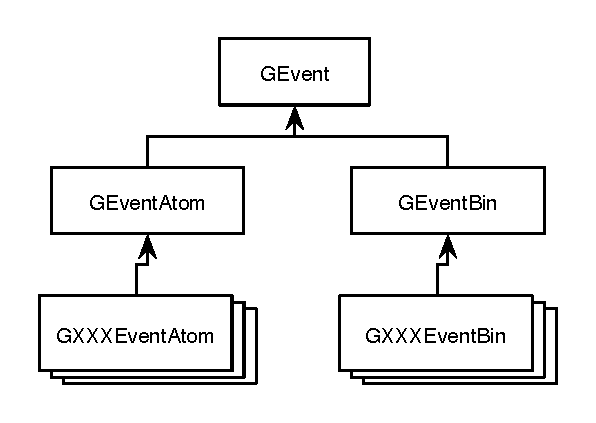
\includegraphics[width=9.1cm]{GEvent.eps}
\caption{Class dependencies for the {\tt GEvent} class.}
\label{fig:GEvent}
\end{figure}
%

The following virtual methods are defined for {\tt GEvent}:
\begin{verbatim}
  double   counts(void) const;                         //!< Number of counts in event
  double   model(GModels& models);                     //!< Model value
  double   model(GModels& models, GVector* gradient);  //!< Model value and gradient
  GTime*   time(void);                                 //!< Time tag of event
  GEnergy* energy(void);                               //!< Event energy
  GSkyDir* dir(void);                                  //!< Arrival direction of event
  bool     isatom(void) const;                         //!< Event is an atom
  bool     isbin(void) const;                          //!< Event is a bin
\end{verbatim}


%%%%%%%%%%%%%%%%%%%%%%%%%%%%%%%%%%%%%%%%%%%%%%%%%%%
\subsubsection{{\tt GEvents}}

The basic element of event handling is the {\tt GEvents} abstract container base class that
contains {\tt GEvent} objects.
The derived abstract container class {\tt GEventList} holds {\tt GEventAtom} objects, 
while the derived abstract container class {\tt GEventCube} holds {\tt GEventBin} objects.
Derived from these two classes are the instrument specific container classes
{\tt GXXXEventList} and {\tt GXXXEventCube} (where {\tt XXX} is the instrument code)
which implement the instrument specific methods.
The class dependencies are shown in Fig.~\ref{fig:GEvents}.
%
%
\begin{figure}[!h]
\centering
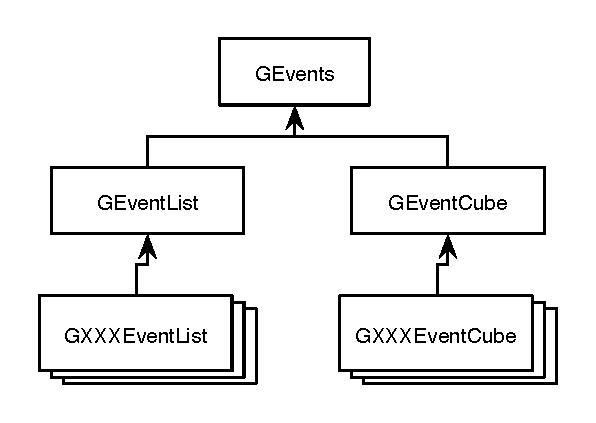
\includegraphics[width=9.1cm]{GEvents.eps}
\caption{Class dependencies for the {\tt GEvents} class.}
\label{fig:GEvents}
\end{figure}
%
%
The following generic methods are implemented:
\begin{verbatim}
  void    load(const std::string& filename);   //!< Load events from FITS file
  GEvent* pointer(int index) const;            //!< Returns pointer to event (atom or bin)
  int     number(void) const;                  //!< Returns total number of events
  int     elements(void) const;                //!< Returns total number of elements
\end{verbatim}
Note that for an event list the total number of elements is identical to the total
number of events.

{\tt GEvents} allows for iterating to provide successive access to events.
The example below shows how iterating is implemented (illustrated using
the {\tt GLATEvents} derived class):
\begin{verbatim}
  GLATEvents events;
  ...
  for (GLATEvents::iterator event = events.begin(); event != events.end(); ++event) {
      cout << *event << endl;
  }
\end{verbatim}


%%%%%%%%%%%%%%%%%%%%%%%%%%%%%%%%%%%%%%%%%%%%%%%%%%%
\subsection{Model handling}

{\tt GModel} desribes how the gamma-ray (or background event) intensity $I$ depends on 
the direction $\vec{d}$ on the sky, on the photon energy $E_{\gamma}$, and on the time 
$t$ as function of a number of parameters $\vec{p}$.
It is assumed that the spatial, spectral and temporal description can be factorized following
\begin{equation}
I(\vec{d},E_{\gamma},t | \vec{p}) = I(\vec{d} | \vec{p}) \times I(E_{\gamma} | \vec{p}) 
\times I(t | \vec{p}) 
\end{equation}


%%%%%%%%%%%%%%%%%%%%%%%%%%%%%%%%%%%%%%%%%%%%%%%%%%%
\subsubsection{{\tt GModelPar}}

The elements of the parameter vector $\vec{p}$ are realized by the {\tt GModelPar} class
\begin{verbatim}
  class GModelPar {
  ...
  protected:
    std::string m_name;      //!< Parameter name
    std::string m_unit;      //!< Parameter unit
    double      m_value;     //!< Parameter value
    double      m_error;     //!< Uncertainty in parameter value
    double      m_min;       //!< Parameter value minimum
    double      m_max;       //!< Parameter value maximum
    double      m_scale;     //!< Parameter scaling (real = m_value * m_scale)
    bool        m_free;      //!< Parameter is free/fixed (for fitting)
    bool        m_hasmin;    //!< Parameter has minimum boundary
    bool        m_hasmax;    //!< Parameter has maximum boundary
  }
\end{verbatim}


%%%%%%%%%%%%%%%%%%%%%%%%%%%%%%%%%%%%%%%%%%%%%%%%%%%
\subsubsection{{\tt GModel}}

The model is realized by the {\tt GModel} class
\begin{verbatim}
  class GModel {
  ...
    std::string name(void) const;               //!< Return model name
    void        name(const std::string& name);  //!< Set model name
    int         npars(void) const;              //!< Returns number of parameters
    GModelPar*  par(int) const;                 //!< Returns pointer to parameter
  protected:
    int             m_npars;        //!< Total number of parameters in model
    GModelPar**     m_par;          //!< Pointers to all model parameters
    GModelSpatial  *m_spatial;      //!< I(d|p)
    GModelSpectral *m_spectral;     //!< I(E|p)
    GModelTemporal *m_temporal;     //!< I(t|p)
  }
\end{verbatim}


%%%%%%%%%%%%%%%%%%%%%%%%%%%%%%%%%%%%%%%%%%%%%%%%%%%
\subsubsection{{\tt GModelSpatial}}

The abstract base class {\tt GModelSpatial} implements different functional forms for 
$I(\vec{d} | \vec{p})$.
The derived classes contain the model parameters, and {\tt m\_par} provides pointers
to all these parameters for quick access.
As an example, the {\tt GModelSpatialPtsrc} derived class is show:
\begin{verbatim}
  class GModelSpatialPtsrc {
  ...
    int        npars(void) const;   //!< Returns number of parameters
    GModelPar* par(int) const;      //!< Returns pointer to parameter
  protected:
    GModelPar  m_ra;                //!< Right Ascension of source
    GModelPar  m_dec;               //!< Declination of source
  }
\end{verbatim}
The following classes are implemented:
\begin{verbatim}
  GModelSpatialPtsrc      //!< Point source
\end{verbatim}


%%%%%%%%%%%%%%%%%%%%%%%%%%%%%%%%%%%%%%%%%%%%%%%%%%%
\subsubsection{{\tt GModelSpectral}}

The abstract base class {\tt GModelSpectral} implements different functional forms for 
$I(E_{\gamma} | \vec{p})$.
The following classes are implemented:
\begin{verbatim}
  GModelSpatialPlaw       //!< Power law
\end{verbatim}


%%%%%%%%%%%%%%%%%%%%%%%%%%%%%%%%%%%%%%%%%%%%%%%%%%%
\subsubsection{{\tt GModelTemporal}}

The abstract base class {\tt GModelTemporal} implements different functional forms for 
$I(t | \vec{p})$.
The following classes are implemented:
\begin{verbatim}
  GModelTemporalConst     //!< Constant source
\end{verbatim}


%%%%%%%%%%%%%%%%%%%%%%%%%%%%%%%%%%%%%%%%%%%%%%%%%%%
\subsubsection{{\tt GModels}}

The models are collected into the {\tt GModels} container class
\begin{verbatim}
  class GModels : public GOptimizerPars {
    void        add(GModel);        //!< Add model to container
    int         npars(void) const;  //!< Returns number of parameters
    GModelPar*  par(int) const;     //!< Returns pointer to parameter
  ...
    int         m_elements;         //!< Total number of models
    GModel*     m_model;            //!< Pointers to all models
    int         m_npars;            //!< Total number of model parameters
    GModelPar** m_par;              //!< Pointers to all model parameters
  }
\end{verbatim}
which is derived from the general parameter container class {\tt GOptimizerPars}.
It is this container class that is handed to {\tt GData} in order to compute the model
prediction for a some given data.
The interpretation of the models is done on the level of the instrument specific classes
{\tt GXXXEventList} and {\tt GXXXEventCube} (where {\tt XXX} is the instrument code).

{\tt GModels} is also handed to the {\tt GOptimizer} class for parameter optimization.

The following code illustrates how a point source is set up for the Crab pulsar with a
power law spectral shape:
\begin{verbatim}
  // Define Crab position
  GSkyDir dir;
  dir.radec_deg(83.6331, +22.0145);
  
  // Spatial model is a point source at the position of the Crab
  GModelSpatialPtsrc point_source = GModelSpatialPtsrc(dir);
  
  // Spectral model is a power law
  GModelSpectralPlaw power_law = GModelSpectralPlaw(1.0e-7, -2.1);
  
  // Set up Crab model
  GModel crab = GModel(point_source, power_law);
  
  // Create model container
  GModels models;
  models.add(crab);
  
  // Set model for observation
  GData data;
  ...
  data.set_model(models);
\end{verbatim}


%%%%%%%%%%%%%%%%%%%%%%%%%%%%%%%%%%%%%%%%%%%%%%%%%%%
\subsection{Optimizer}

%%%%%%%%%%%%%%%%%%%%%%%%%%%%%%%%%%%%%%%%%%%%%%%%%%%
\subsubsection{{\tt GOptimizerFunction}}

The abstract base class {\tt GOptimizerFunction} provides the interface between any
user-defined function and the {\tt GOptimizer} class.
The {\tt GOptimizerFunction} class has the following structure:
\begin{verbatim}
  class GOptimizerFunction {
    ...
    virtual void           eval(const GOptimizerPars& pars); //!< Evaluate function
    virtual double*        value(void);        //!< Return pointer to function value
    virtual GVector*       gradient(void);     //!< Return pointer to gradient
    virtual GSparseMatrix* covar(void);        //!< Return pointer to covariance matrix
  }
\end{verbatim}




%%%%%%%%%%%%%%%%%%%%%%%%%%%%%%%%%%%%%%%%%%%%%%%%%%%
\subsubsection{{\tt GOptimizer}}

The {\tt GOptimizer} class ...
\begin{verbatim}
  class GOptimizer {
    ...
    virtual GOptimizerPars& operator() (GOptimizerFunction& fct, GOptimizerPars& p);
    GModels& operator() (GOptimizerFunction& fct, GModels& m);
    }
  }
\end{verbatim}

Optimization is then done using

\begin{verbatim}
  void GData::optimize(GOptimizer& opt)
  {
    // Set optimizer function
    GData::optimizer fct(this);

    // Optimise model parameters
    m_models = opt(fct, m_models);

    // Return
    return;
  }
\end{verbatim}



%%%%%%%%%%%%%%%%%%%%%%%%%%%%%%%%%%%%%%%%%%%%%%%%%%%
% User Interface Design
%%%%%%%%%%%%%%%%%%%%%%%%%%%%%%%%%%%%%%%%%%%%%%%%%%%
\section{User Interface Design}

%%%%%%%%%%%%%%%%%%%%%%%%%%%%%%%%%%%%%%%%%%%%%%%%%%%
\subsection{Description of the User Interface}


%%%%%%%%%%%%%%%%%%%%%%%%%%%%%%%%%%%%%%%%%%%%%%%%%%%
% Additional Material
%%%%%%%%%%%%%%%%%%%%%%%%%%%%%%%%%%%%%%%%%%%%%%%%%%%
\section{Additional Material}

\end{document} 
